\documentclass[a4paper,12pt,twoside]{report}

\usepackage[left=3cm,right=3cm,top=3cm,bottom=3cm]{geometry} %Margins
\usepackage{pdfpages}
\usepackage{hyperref}
\usepackage{listings}
\usepackage{xcolor}
\usepackage{setspace}
\usepackage{tocloft}
\usepackage{amsmath}
\usepackage{chngcntr }
\usepackage[toc,page]{appendix}
\usepackage[T1]{fontenc}
\usepackage[nottoc]{tocbibind}
\usepackage[compact]{titlesec}
\usepackage{float}

\usepackage[utf8]{inputenc}
\usepackage{amsmath, amssymb, latexsym}
\usepackage{sidecap}

%---tikz---

\usepackage{tikz}
\usetikzlibrary{decorations.pathreplacing}
\usetikzlibrary{fadings}
\usetikzlibrary{positioning}

\titlespacing{\section}{0pt}{1ex}{0ex}
\titlespacing{\subsection}{0pt}{1ex}{0ex}
\titlespacing{\subsubsection}{0pt}{1ex}{0ex}

\counterwithout{figure}{chapter}
\counterwithout{table}{chapter}

\usepackage{graphicx}
\usepackage{verbatim}
\usepackage{latexsym}
\usepackage{mathchars}
\usepackage{setspace}
\usepackage{blindtext}
\usepackage{float}

\setlength{\parskip}{\medskipamount}  % a little space before a \par
\setlength{\parindent}{0pt}	% don't indent first lines of paragraphs
%UHEAD.STY  If this is included after \documentstyle{report}, it adds
% an underlined heading style to the LaTeX report style.
% \pagestyle{uheadings} will put underlined headings at the top
% of each page. The right page headings are the Chapter titles and
% the left page titles are supplied by \def\lefthead{text}.

% Ted Shapin, Dec. 17, 1986

\makeatletter
\def\chapapp2{Chapter}

\def\appendix{\par
 \setcounter{chapter}{0}
 \setcounter{section}{0}
 \def\chapapp2{Appendix}
 \def\@chapapp{Appendix}
 \def\thechapter{\Alph{chapter}}}

\def\ps@uheadings{\let\@mkboth\markboth
% modifications
\def\@oddhead{\protect\underline{\protect\makebox[\textwidth][l]
		{\sl\rightmark\hfill\rm\thepage}}}
\def\@oddfoot{}
\def\@evenfoot{}
\def\@evenhead{\protect\underline{\protect\makebox[\textwidth][l]
		{\rm\thepage\hfill\sl\leftmark}}}
% end of modifications
\def\chaptermark##1{\markboth {\ifnum \c@secnumdepth >\m@ne
 \chapapp2\ \thechapter. \ \fi ##1}{}}%
\def\sectionmark##1{\markright {\ifnum \c@secnumdepth >\z@
   \thesection. \ \fi ##1}}}
\makeatother
%%From: marcel@cs.caltech.edu (Marcel van der Goot)
%%Newsgroups: comp.text.tex
%%Subject: illegal modification of boxit.sty
%%Date: 28 Feb 92 01:10:02 GMT
%%Organization: California Institute of Technology (CS dept)
%%Nntp-Posting-Host: andromeda.cs.caltech.edu
%%
%%
%%Quite some time ago I posted a file boxit.sty; maybe it made it
%%to some archives, although I don't recall submitting it. It defines
%%	\begin{boxit}
%%	...
%%	\end{boxit}
%%to draw a box around `...', where the `...' can contain other
%%environments (e.g., a verbatim environment). Unfortunately, it had
%%a problem: it did not work if you used it in paragraph mode, i.e., it
%%only worked if there was an empty line in front of \begin{boxit}.
%%Luckily, that is easily corrected.
%%
%%HOWEVER, apparently someone noticed the problem, tried to correct it,
%%and then distributed this modified version. That would be fine with me,
%%except that:
%%1. There was no note in the file about this modification, it only has my
%%   name in it.
%%2. The modification is wrong: now it only works if there is *no* empty
%%   line in front of \begin{boxit}. In my opinion this bug is worse than
%%   the original one.
%%
%%In particular, the author of this modification tried to force an empty
%%line by inserting a `\\' in the definition of \Beginboxit. If you have
%%a version of boxit.sty with a `\\', please delete it. If you have my
%%old version of boxit.sty, please also delete it. Below is an improved
%%version.
%%
%%Thanks to Joe Armstrong for drawing my attention to the bug and to the
%%illegal version.
%%
%%                                          Marcel van der Goot
%% .---------------------------------------------------------------
%% | Blauw de viooltjes,                    marcel@cs.caltech.edu
%% |    Rood zijn de rozen;
%% | Een rijm kan gezet
%% |    Met plaksel en dozen.
%% |


% boxit.sty
% version: 27 Feb 1992
%
% Defines a boxit environment, which draws lines around its contents.
% Usage:
%   \begin{boxit}
%	... (text you want to be boxed, can contain other environments)
%   \end{boxit}
%
% The width of the box is the width of the contents.
% The boxit* environment behaves the same, except that the box will be
% at least as wide as a normal paragraph.
%
% The reason for writing it this way (rather than with the \boxit#1 macro
% from the TeXbook), is that now you can box verbatim text, as in
%   \begin{boxit}
%   \begin{verbatim}
%   this better come out in boxed verbatim mode ...
%   \end{verbatim}
%   \end{boxit}
%
%						Marcel van der Goot
%						marcel@cs.caltech.edu
%

\def\Beginboxit
   {\par
    \vbox\bgroup
	   \hrule
	   \hbox\bgroup
		  \vrule \kern1.2pt %
		  \vbox\bgroup\kern1.2pt
   }

\def\Endboxit{%
			      \kern1.2pt
		       \egroup
		  \kern1.2pt\vrule
		\egroup
	   \hrule
	 \egroup
   }	

\newenvironment{boxit}{\Beginboxit}{\Endboxit}
\newenvironment{boxit*}{\Beginboxit\hbox to\hsize{}}{\Endboxit}
\pagestyle{empty}

\setlength{\parskip}{2ex plus 0.5ex minus 0.2ex}
\setlength{\parindent}{0pt}

\makeatletter  %to avoid error messages generated by "\@". Makes Latex treat "@" like a letter

\linespread{1.5}
\def\submitdate#1{\gdef\@submitdate{#1}}
\def\supervisor#1{\gdef\@supervisor{#1}}
\def\cosupervisor#1{\gdef\@cosupervisor{#1}}

\def\maketitle{
  % Title
  \begin{titlepage}{
    \vspace*{2\baselineskip} %Empty Lines
    {\fontsize{17.28}{16.8}\selectfont Master thesis in Sound and Music Computing}\\
     {\fontsize{14}{16.8}\selectfont Epidemic Sound and Universitat Pompeu Fabra}\\
    \rm
    \vspace*{3\baselineskip} %Empty Lines
     \bf \fontsize{24.88}{17.5}\selectfont  \@title \par
  }
  \vskip 0.3in
  \par
  {\fontsize{14}{27}\selectfont  \@author}

  \vskip 0.20in
  \fontsize{14}{16.8}\selectfont \textbf{Supervisor:}   \@supervisor \\
  \fontsize{14}{16.8}\selectfont \textbf{Co-Supervisor:}  \@cosupervisor \\
   \vspace*{3\baselineskip} %Empty Lines
    \fontsize{14}{27}\selectfont  \@submitdate \\
    \vspace{ 0.7in}
    
\includegraphics[width=8cm]{Figures/LogoEpidemicSound.png}\\[.5cm]
    
\includegraphics[width=8cm]{Figures/LogoPompeuFabra}\\[.5cm]
  \vfil
  \end{titlepage}
}

\def\titlepage{
  \newpage
  \centering
  \linespread{1.5}
  \normalsize
  \vbox to \vsize\bgroup\vbox to 9in\bgroup
}
\def\endtitlepage{
  \par
  \kern 0pt
  \egroup
  \vss
  \egroup
  \cleardoublepage
}

\def\abstract{
  \begin{center}{
    \large\bf Abstract}
  \end{center}
  \small
  %\def\baselinestretch{1.5}
  \linespread{1.5}
  \normalsize
}
\def\endabstract{
  \par
   \cleardoublepage
}

\newenvironment{acknowledgement}{
  \clearpage
  \begin{center}{
    \large \bf Acknowledgement}
  \end{center}
  \small
  \linespread{1.5}
  \normalsize
}{\clearpage}
\def\endacknowledgement{
  \par
    \cleardoublepage
}

\newenvironment{dedication}{
  \clearpage
  \begin{center}{
    \large \bf Dedication}
  \end{center}
  \small
  \linespread{1.5}
  \normalsize
}{\clearpage}
\def\enddedication{
  \par
  \cleardoublepage
}

\def\preface{
    \pagenumbering{gobble}
    \pagestyle{plain}
    \doublespacing
     \setcounter{tocdepth}{2}
    \tableofcontents
}

\def\body{

    \clearpage    
    \pagestyle{uheadings}
    \pagenumbering{arabic}
    \singlespacing  
    \setlength{\cftbeforesecskip}{10pt}

    \pagestyle{plain}
    \clearpage
    \pagestyle{uheadings}
    
}

\makeatother  %to avoid error messages generated by "\@". Makes Latex treat "@" like a letter

\newcommand{\titlelinespacing}{\renewcommand{\baselinestretch}{2.0} \normalsize}
\newcommand{\normallinespacing}{\renewcommand{\baselinestretch}{1.5} \normalsize}
\newcommand{\mediumlinespacing}{\renewcommand{\baselinestretch}{1.2} \normalsize}
\newcommand{\narrowlinespacing}{\renewcommand{\baselinestretch}{1.0} \normalsize}

\newtheorem{definition}{Definition}[chapter]
\newtheorem{theorem}{Theorem}[chapter]
\cftsetindents{section}{0in}{0.5in}
\cftsetindents{subsection}{0in}{0.5in}
\cftsetindents{subsubsection}{0in}{0.5in}
\cftsetindents{paragraph}{0in}{0.5in}


\begin{document}

\newgeometry{left=2cm,right=2cm} %Only for the title new margins

%Title parameters
\title{%
  Uncovering underlying musical content in the temporal domain \\
  \small Leveraging deep learning, inductive bias, and aural skills to learn embedding spaces from raw waveforms with applications to MIR downstream tasks}
  
\author{\href{oriol.colome.font@epidemicsound.com}{Oriol Colomé Font}}
\submitdate{July 2023}
\supervisor{Carlos Lordelo and Carl Thomé}
\cosupervisor{Frederic Font}

\hypersetup{
pdftitle={Your PDF title},
pdfsubject={Your PDF subject},
pdfauthor={Oriol Colomé Font},
pdfkeywords={Music; 
Music Theory; 
Music Information Retrieval; 
Music Structure Analysis; 
Machine Learning; 
Neural Networks; 
Deep Learning}
}

\maketitle

\restoregeometry

\preface
\cleardoublepage 

%\addcontentsline{toc}{chapter}{Acknowledgement}
\begin{dedication}
\pagenumbering{gobble}% Remove page numbers (and reset to 1)
(Optional, if used placed on a right page next to an empty left page)

I would like to dedicate this work to...
\newpage

\end{dedication}


%\addcontentsline{toc}{chapter}{Acknowledgement}

\begin{acknowledgement}
\pagenumbering{gobble}% Remove page numbers (and reset to 1)

I want to extend my deepest gratitude to...

\begin{itemize}
\item Carlos Lordelo and Carl Thomé for their invaluable guidance and support throughout my thesis. Their MIR, ML, and DSP expertise has been instrumental in shaping my research and driving it toward success. I am truly grateful for their unwavering support and encouragement, which helped me surmount any difficulties I encountered during this journey. Their time, effort, and dedication in mentoring me have not gone unnoticed. They inspire me with their commitment to their students, and I feel honored to have had the opportunity to work with them.

Words fall short of my profound gratitude for their consistent, knowledgeable, and steadfast support. I am beyond grateful that their dedication has left an indelible mark on my academic journey.

\vspace*{3mm}
\item Cody Hesse and Sebastian Löf
\vspace*{3mm}
\item Epidemic Sound AB (\textit{Aktiebolag})
\vspace*{3mm}
\item My co-supervisor
\vspace*{3mm}
\item The Music Technology Group (MTG)
\vspace*{3mm}
\item My colleague at My Sheet Music Transcriptions, Oriol López, for his exceptional support and flexibility throughout my thesis. His understanding and willingness to accommodate my academic commitments effectively allowed me to balance my work and research responsibilities. I am genuinely grateful for his unwavering support and encouragement.
\vspace*{3mm}
Thank you all for being excellent advisors and playing a crucial role in completing my thesis. I sincerely appreciate everything you have done for me and will always cherish the knowledge and experience I have gained under your guidance.
\vspace*{3mm}
\end{itemize}

\newpage
\end{acknowledgement}
%\addcontentsline{toc}{chapter}{Acknowledgement}
\begin{preface}
\pagenumbering{gobble}% Remove page numbers (and reset to 1)

Music and science have always been my two greatest passions. When the opportunity to work at Epidemic Sound presented itself, it was as if the universe had conspired to bring my interests together, offering me the chance to explore the fascinating field of MIR from an industrial perspective. With the support and encouragement of my loved ones, I took a leap of faith and moved to Stockholm to embark on this exciting journey.

This work aims to help untangle the complexities of music and offer a more musically-driven perspective to MIR. I aim to contribute to a deeper understanding of the intricate relationships within musical data by bridging the gap between music theory and computational analysis.

I am deeply grateful to the Epidemic Sound team for their guidance, expertise, and camaraderie throughout this project. I would also like to extend my heartfelt appreciation to my family for their unwavering support and belief in my abilities.

My motivation for writing this piece stems from a desire to grow as a musician, programmer, professional, and individual. I believe that by delving into the world of MIR, I can expand my horizons while making a meaningful contribution to the field.

This work is intended for any curious human being, regardless of their background in music or computer science. I hope it will inspire others to explore the captivating intersection of these two disciplines.

The scope of this work encompasses a range of MIR tasks and methodologies, as well as discussions on the challenges and opportunities that arise within the field. Despite the ambitious nature of this project, I acknowledge that time and my academic background limitations may have constrained the depth of my analysis. Nevertheless, I hope this work will serve as a starting point for further exploration and inspire new ideas in the realm of MIR.

\newpage
\end{preface}
%\addcontentsline{toc}{chapter}{Abstract}

\begin{abstract}
\pagenumbering{gobble}

Music, an integral part of human culture, offers a diverse yet complex field of study due to its intricate styles, mutable ground truth, and subjective nature. This research, conducted in collaboration with Epidemic Sound AB and the Music Technology Group (MTG) at Universitat Pompeu Fabra (UPF), employs self-supervised contrastive learning of musical representation to uncover the fundamental structure of Western tonal music. 

Embracing a subtle novel approach, this process is facilitated by applying Siamese networks with a triplet loss, mimicking human aural skills in interpreting music to discern abstract and semantic musical elements, irrespective of the sonic qualities. The study replaces traditional acoustical features with deep audio embeddings to compute high-level, sound-agnostic, and content-sensitive music identification.

Results XXXXXX TBC

The preliminary results suggest that our approach to learning music-informed embeddings holds significant potential for nearly all MIR downstream tasks. Music-motivated embeddings represent a promising technique, adaptable potentially to other tasks hindered by data scarcity. This method could significantly influence advancements in intelligent music recommendation systems and the efficient enforcement of intellectual property rights. 

\bigskip
Keywords: Music Information Retrieval; Music Structure Analysis; Deep Audio Embeddings, Aural Skills

\newpage
\end{abstract}

\body

%Introduction of the project
\normallinespacing

\chapter{Introduction}

This master thesis investigates the interrelationship between music\footnote{The term "music" used in this context refers specifically to Western tonal music tradition. It is assumed that the musical structures and elements discussed are based on this tradition and may not apply to other musical styles or cultures.} structure analysis, aural skills, and the underlying musical structure in musical composition. 

Musical elements, including melody, harmony, rhythm, and form, constitute music structure analysis. 

Aural skills encompass perceptual and cognitive abilities, enabling individuals to comprehend musical works through listening. These skills encompass the ability to differentiate musical elements, comprehend relationships between them, and discern the structure of a musical composition. 

The underlying musical structure refers to the systematic arrangement of musical elements that results in a coherent and expressive musical work. 

This master thesis investigates the interplay between music structure analysis, aural skills, and the underlying musical structure through a comprehensive analysis of musical works from diverse styles and genres. By utilizing computational techniques from Music Information Retrieval (MIR) and incorporating a musicological perspective to contextualize the findings, this thesis aspires to offer a fresh and insightful examination of these components of musical composition and further our understanding of their relationships.

\section{Motivation}

As a music lover and connoisseur, I am interested in gaining a deeper understanding of the fundamental building of musical composition, the various techniques used to create musical works, and capturing underlying relationships among them. I am deeply interested in learning how to retrieve embedded information within music. The study of music structure analysis provides a means to systematically analyze and understand musical pieces. It has traditionally been approached through music theory, formal musical notation, musical analysis techniques, and machine learning, which I plan to blend.

With the advent of artificial intelligence and machine learning, Music Information Retrieval (MIR) has expanded to encompass musically motivated neural network architectures. These networks are designed to incorporate musical concepts and perceptual approaches and use this knowledge to analyze and understand the structure of musical pieces in a way that goes beyond traditional music analysis techniques.

As a professional musician and music transcriber, I am interested in understanding how deep neural networks (DNNs) filter musical features. In other words, I am eager to learn how DNNs listen~\cite{7500246} to music.

By studying music structure analysis using musically motivated neural networks, we will gain an in-depth understanding of the latest advancements in the field and how these techniques are being used to revolutionize our understanding of music. Additionally, we will be able to contribute to developing new and innovative methods for musical analysis~\cite{Huang2019MusicTG}

\section{Objectives}

As a professional music transcriber, I aim to understand how deep neural networks (DNNs) filter musical features, listen to the NN layers from a musician's perspective and analyze the resulting data. I aim to approach the technology from a technical and musical standpoint to understand how DNNs process and extract musical information. By doing so, I aim to enhance the accuracy and efficiency of the process and contribute to developing AI technology for music analysis. By combining my expertise in music with my -not fully developed- knowledge of DNNs, I hope to bring a unique perspective to the field and contribute to the advancement of music analysis.

Music is a complex and multi-faceted phenomenon, and implementing a model that mimics human aural music skills is challenging. However, using the latest deep learning techniques, we aim to build a model that achieves good results for a specific task in the domain of music.

\section{Structure of the Report}

In this report, we have organized the information into several sections and sub-sections to provide a clear and comprehensive overview of the topic. The structure of the report is as follows:

\begin{itemize}
\item Chapter 1
  \begin{itemize}
  \item Purpose
  \item Methodology
  \item Scope
  \end{itemize}
\item Chapter 2
  \begin{itemize}
  \item Section 1
  \item Section 2
  \item Section 3
  \end{itemize}
\item Chapter 3
  \begin{itemize}
  \item Summary
  \item Recommendations
  \end{itemize}
\item References
  \begin{itemize}
  \item Sources Cited
  \end{itemize}
\end{itemize}

\newpage



%Task definition
%%\input{task definition}
%Methods
\chapter{Methods}

\section{Materials}

\section{Convolutional Neural Network (CNN)}

A Convolutional Neural Network (CNN), is a deep-learning neural network. The architecture of a CNN is composed of several layers, including:

\begin{itemize}

\item Convolutional layers: These layers apply a convolution operation to the input data, effectively learning local patterns and features in the image. The raw audio data is typically transformed into a spectrogram or a Mel-spectrogram representation, which can be considered an image-like 2D representation of the audio data. The convolutional layers are designed to learn local patterns and features in the audio data
\vspace*{3mm}

\item Pooling layers: These layers downsample the data, reducing the spatial dimensions of the input while retaining important information. They can also be used to downsample the data and reduce the temporal dimensions of the input while retaining important information. 
\vspace*{3mm}

\item Fully connected layers: These layers connect every neuron in one layer to every neuron in another layer, allowing the network to learn non-linear combinations of the features learned in the previous layers.
\vspace*{3mm}

\item Output layer: The output layer produces the final predictions of the network.
\end{itemize}

Compared to a traditional neural network, CNNs are more computationally efficient and have less number of parameters to train. This makes them more feasible for large-scale datasets and real-world problems.

On top of that, one of the main advantages of using CNNs for audio analysis is that they can automatically and adaptively learn temporal hierarchies of features from audio data, which traditional audio processing methods may not be able to do effectively. 

\subsection{Neural Network (NN)}

%Single
\begin{SCfigure}[2\sidecaptionrelwidth][h]
	\centering
	\begin{tikzpicture}[shorten >=1pt,->]
		\tikzstyle{unit}=[draw,shape=circle,minimum size=1.15cm]
 
		\node[unit](p) at (2,1){$y$};
		\node(dots) at (-0.25,1){\vdots};
 
		\draw (0,2.5) node[xshift=-10]{$w_0$} -- (p);
		\draw (0,1.75) node[xshift=-10]{$x_1$} --(p);
		\draw (0,0) node[xshift=-10]{$x_D$} -- (p);
		\draw (p) -- (3,1) node[xshift=30]{$y := f(z)$};
	\end{tikzpicture}
	\caption[Single processing units and its components.]{Single processing unit and its components. The activation function is denoted by $f$ and applied to the actual input $z$ of the unit to form its output $y = f(z)$. $x_1, \ldots, x_D$ represent input from other units within the network; $w_0$ is called bias and represents an external input to the unit. All inputs are mapped onto the actual input $z$ using the propagation rule.}
	\label{fig:processing-unit}
\end{SCfigure}
%NN
\begin{SCfigure}[12][h]
	\centering
    \begin{tikzpicture}[shorten >=1pt]
        \tikzstyle{unit}=[draw,shape=circle,minimum size=1.15cm]
 
        \node[unit](x0) at (0,3.5){$x_0$};
        \node[unit](x1) at (0,2){$x_1$};
        \node(dots) at (0,1){\vdots};
        \node[unit](xd) at (0,0){$x_D$};
 
        \node[unit](y1) at (4,2.5){$y_1$};
        \node(dots) at (4,1.5){\vdots};
        \node[unit](yc) at (4,0.5){$y_C$};
 
        \draw[->] (x0) -- (y1);
        \draw[->] (x0) -- (yc);
 
        \draw[->] (x1) -- (y1);
        \draw[->] (x1) -- (yc);
 
        \draw[->] (xd) -- (y1);
        \draw[->] (xd) -- (yc);
 
        \draw [decorate,decoration={brace,amplitude=10pt},xshift=-4pt,yshift=0pt] (-0.5,4) -- (0.75,4) node [black,midway,yshift=+0.6cm]{input layer};
        \draw [decorate,decoration={brace,amplitude=10pt},xshift=-4pt,yshift=0pt] (3.5,3) -- (4.75,3) node [black,midway,yshift=+0.6cm]{output layer};
    \end{tikzpicture}
    \caption[Network graph of a perceptron with $D$ input units and $C$ output units.]{The perceptron consists of $D$ input units and $C$ output units. All units are labeled according to their output: $y_i = f(z_i)$ in the case of output units; $x_i$ in the case of input units. The input values $x_i$ are propagated to each output unit using the weighted sum propagation rule. The additional input value $x_0 := 1$ is used to include the biases as weights.}
    \label{fig:perceptron}
\end{SCfigure}

%Backpropagation
\begin{figure}[h]
	\centering
	\begin{tikzpicture}[shorten >=1pt]
		\tikzstyle{unit}=[draw,shape=circle,minimum size=1.15cm]
		%\tikzstyle{hidden}=[draw,shape=circle,fill=black!25,minimum size=1.15cm]
		\tikzstyle{hidden}=[draw,shape=circle,minimum size=1.15cm]
 
		\node[unit](x0) at (0,3.5){$x_0$};
		\node[unit](x1) at (0,2){$x_1$};
		\node at (0,1){\vdots};
		\node[unit](xd) at (0,0){$x_D$};
 
		\node[hidden](h10) at (3,4){$y_0^{(1)}$};
		\node[hidden](h11) at (3,2.5){$y_1^{(1)}$};
		\node at (3,1.5){\vdots};
		\node[hidden](h1m) at (3,-0.5){$y_{m^{(1)}}^{(1)}$};
 
		\node(h22) at (5,0){};
		\node(h21) at (5,2){};
		\node(h20) at (5,4){};
		
		\node(d3) at (6,0){$\ldots$};
		\node(d2) at (6,2){$\ldots$};
		\node(d1) at (6,4){$\ldots$};
 
		\node(hL12) at (7,0){};
		\node(hL11) at (7,2){};
		\node(hL10) at (7,4){};
		
		\node[hidden](hL0) at (9,4){$y_0^{(L)}$};
		\node[hidden](hL1) at (9,2.5){$y_1^{(L)}$};
		\node at (9,1.5){\vdots};
		\node[hidden](hLm) at (9,-0.5){$y_{m^{(L)}}^{(L)}$};
 
		\node[unit](y1) at (12,3.5){$y_1^{(L+1)}$};
		\node[unit](y2) at (12,2){$y_2^{(L+1)}$};
		\node at (12,1){\vdots};	
		\node[unit](yc) at (12,0){$y_C^{(L+1)}$};
 
		\draw[->] (x0) -- (h11);
		\draw[->] (x0) -- (h1m);
 
		\draw[->] (x1) -- (h11);
		\draw[->] (x1) -- (h1m);
 
		\draw[->] (xd) -- (h11);
		\draw[->] (xd) -- (h1m);
 
		\draw[->] (hL0) -- (y1);
		\draw[->] (hL0) -- (yc);
		\draw[->] (hL0) -- (y2);
 
		\draw[->] (hL1) -- (y1);
		\draw[->] (hL1) -- (yc);
		\draw[->] (hL1) -- (y2);
 
		\draw[->] (hLm) -- (y1);
		\draw[->] (hLm) -- (y2);
		\draw[->] (hLm) -- (yc);
 
		\draw[->,path fading=east] (h10) -- (h21);
		\draw[->,path fading=east] (h10) -- (h22);
		
		\draw[->,path fading=east] (h11) -- (h21);
		\draw[->,path fading=east] (h11) -- (h22);
		
		\draw[->,path fading=east] (h1m) -- (h21);
		\draw[->,path fading=east] (h1m) -- (h22);
		
		\draw[->,path fading=west] (hL10) -- (hL1);
		\draw[->,path fading=west] (hL11) -- (hL1);
		\draw[->,path fading=west] (hL12) -- (hL1);
		
		\draw[->,path fading=west] (hL10) -- (hLm);
		\draw[->,path fading=west] (hL11) -- (hLm);
		\draw[->,path fading=west] (hL12) -- (hLm);
		
		\draw [decorate,decoration={brace,amplitude=10pt},xshift=-4pt,yshift=0pt] (-0.5,4) -- (0.75,4) node [black,midway,yshift=+0.6cm]{input layer};
		\draw [decorate,decoration={brace,amplitude=10pt},xshift=-4pt,yshift=0pt] (2.5,4.5) -- (3.75,4.5) node [black,midway,yshift=+0.6cm]{$1^{\text{st}}$ hidden layer};
		\draw [decorate,decoration={brace,amplitude=10pt},xshift=-4pt,yshift=0pt] (8.5,4.5) -- (9.75,4.5) node [black,midway,yshift=+0.6cm]{$L^{\text{th}}$ hidden layer};
		\draw [decorate,decoration={brace,amplitude=10pt},xshift=-4pt,yshift=0pt] (11.5,4) -- (12.75,4) node [black,midway,yshift=+0.6cm]{output layer};
	\end{tikzpicture}
	\caption[Network graph for a $(L+1)$-layer perceptron.]{Network graph of a $(L+1)$-layer perceptron with $D$ input units and $C$ output units. The $l^{\text{th}}$ hidden layer contains $m^{(l)}$ hidden units.}
	\label{fig:multilayer-perceptron}
\end{figure}

%CNN
A high-level illustration of a simple convolutional neural network indicating convolutional layers, pooling layers, and fully-connected layers without details (number of channels or neurons per layer or the input image size) can be seen in XXX.
\begin{figure}[h]
	\centering
	\begin{tikzpicture}
		\node at (0.5,-1){\begin{tabular}{c}input image\\layer $l = 0$\end{tabular}};
		
		\draw (0,0) -- (1,0) -- (1,1) -- (0,1) -- (0,0);
		
		\node at (3,3.5){\begin{tabular}{c}convolutional layer\\with non-linearities\\layer $l = 1$\end{tabular}};
		
		\draw[fill=black,opacity=0.2,draw=black] (2.75,1.25) -- (3.75,1.25) -- (3.75,2.25) -- (2.75,2.25) -- (2.75,1.25);
		\draw[fill=black,opacity=0.2,draw=black] (2.5,1) -- (3.5,1) -- (3.5,2) -- (2.5,2) -- (2.5,1);
		\draw[fill=black,opacity=0.2,draw=black] (2.25,0.75) -- (3.25,0.75) -- (3.25,1.75) -- (2.25,1.75) -- (2.25,0.75);
		\draw[fill=black,opacity=0.2,draw=black] (2,0.5) -- (3,0.5) -- (3,1.5) -- (2,1.5) -- (2,0.5);
		\draw[fill=black,opacity=0.2,draw=black] (1.75,0.25) -- (2.75,0.25) -- (2.75,1.25) -- (1.75,1.25) -- (1.75,0.25);
		\draw[fill=black,opacity=0.2,draw=black] (1.5,0) -- (2.5,0) -- (2.5,1) -- (1.5,1) -- (1.5,0);
		
		\node at (4.5,-1){\begin{tabular}{c}subsampling layer\\layer $l = 3$\end{tabular}};
		
		\draw[fill=black,opacity=0.2,draw=black] (5,1.25) -- (5.75,1.25) -- (5.75,2) -- (5,2) -- (5,1.25);
		\draw[fill=black,opacity=0.2,draw=black] (4.75,1) -- (5.5,1) -- (5.5,1.75) -- (4.75,1.75) -- (4.75,1);
		\draw[fill=black,opacity=0.2,draw=black] (4.5,0.75) -- (5.25,0.75) -- (5.25,1.5) -- (4.5,1.5) -- (4.5,0.75);
		\draw[fill=black,opacity=0.2,draw=black] (4.25,0.5) -- (5,0.5) -- (5,1.25) -- (4.25,1.25) -- (4.25,0.5);
		\draw[fill=black,opacity=0.2,draw=black] (4,0.25) -- (4.75,0.25) -- (4.75,1) -- (4,1) -- (4,0.25);
		\draw[fill=black,opacity=0.2,draw=black] (3.75,0) -- (4.5,0) -- (4.5,0.75) -- (3.75,0.75) -- (3.75,0);
		
		\node at (7,3.5){\begin{tabular}{c}convolutional layer\\with non-linearities\\layer $l = 4$\end{tabular}};
		
		\draw[fill=black,opacity=0.2,draw=black] (7.5,1.75) -- (8.25,1.75) -- (8.25,2.5) -- (7.5,2.5) -- (7.5,1.75);
		\draw[fill=black,opacity=0.2,draw=black] (7.25,1.5) -- (8,1.5) -- (8,2.25) -- (7.25,2.25) -- (7.25,1.5);
		\draw[fill=black,opacity=0.2,draw=black] (7,1.25) -- (7.75,1.25) -- (7.75,2) -- (7,2) -- (7,1.25);
		\draw[fill=black,opacity=0.2,draw=black] (6.75,1) -- (7.5,1) -- (7.5,1.75) -- (6.75,1.75) -- (6.75,1);
		\draw[fill=black,opacity=0.2,draw=black] (6.5,0.75) -- (7.25,0.75) -- (7.25,1.5) -- (6.5,1.5) -- (6.5,0.75);
		\draw[fill=black,opacity=0.2,draw=black] (6.25,0.5) -- (7,0.5) -- (7,1.25) -- (6.25,1.25) -- (6.25,0.5);
		\draw[fill=black,opacity=0.2,draw=black] (6,0.25) -- (6.75,0.25) -- (6.75,1) -- (6,1) -- (6,0.25);
		\draw[fill=black,opacity=0.2,draw=black] (5.75,0) -- (6.5,0) -- (6.5,0.75) -- (5.75,0.75) -- (5.75,0);
		
		\node at (9.5,-1){\begin{tabular}{c}subsampling layer\\layer $l = 6$\end{tabular}};
		
		\draw[fill=black,opacity=0.2,draw=black] (10,1.75) -- (10.5,1.75) -- (10.5,2.25) -- (10,2.25) -- (10,1.75);
		\draw[fill=black,opacity=0.2,draw=black] (9.75,1.5) -- (10.25,1.5) -- (10.25,2) -- (9.75,2) -- (9.75,1.5);
		\draw[fill=black,opacity=0.2,draw=black] (9.5,1.25) -- (10,1.25) -- (10,1.75) -- (9.5,1.75) -- (9.5,1.25);
		\draw[fill=black,opacity=0.2,draw=black] (9.25,1) -- (9.75,1) -- (9.75,1.5) -- (9.25,1.5) -- (9.25,1);
		\draw[fill=black,opacity=0.2,draw=black] (9,0.75) -- (9.5,0.75) -- (9.5,1.25) -- (9,1.25) -- (9,0.75);
		\draw[fill=black,opacity=0.2,draw=black] (8.75,0.5) -- (9.25,0.5) -- (9.25,1) -- (8.75,1) -- (8.75,0.5);
		\draw[fill=black,opacity=0.2,draw=black] (8.5,0.25) -- (9,0.25) -- (9,0.75) -- (8.5,0.75) -- (8.5,0.25);
		\draw[fill=black,opacity=0.2,draw=black] (8.25,0) -- (8.75,0) -- (8.75,0.5) -- (8.25,0.5) -- (8.25,0);
		
		\node at (12,3.5){\begin{tabular}{c}fully connected layer\\layer $l = 7$\end{tabular}};
		
		\draw[fill=black,draw=black,opacity=0.5] (10.5,0) -- (11,0) -- (12.5,1.75) -- (12,1.75) -- (10.5,0);
		
		\node at (13,-1){\begin{tabular}{c}fully connected layer\\output layer $l = 8$\end{tabular}};
		
		\draw[fill=black,draw=black,opacity=0.5] (12.5,0.5) -- (13,0.5) -- (13.65,1.25) -- (13.15,1.25) -- (12.5,0.5);
	\end{tikzpicture}
	\caption[Architecture of a traditional convolutional neural network.]{The architecture of the original convolutional neural network, as introduced by LeCun et al. (1989), alternates between convolutional layers, including hyperbolic tangent non-linearities and subsampling layers. In this illustration, the convolutional layers already include non-linearities and, thus, a convolutional layer represents two layers. The feature maps of the final subsampling layer are then fed into the actual classifier consisting of an arbitrary number of fully connected layers. The output layer usually uses softmax activation functions.}
	\label{fig:traditional-convolutional-network}
\end{figure}

%Single CNN
\begin{SCfigure}[2\sidecaptionrelwidth][h]
	\centering
	\begin{tikzpicture}
		\node at (1.5,4){\begin{tabular}{c}input image\\or input feature map\end{tabular}};
	
		\draw (0,0) -- (3,0) -- (3,3) -- (0,3) -- (0,0);
		
		\draw (2,2) -- (2.5,2) -- (2.5,2.5) -- (2,2.5) -- (2,2);
		\draw (2,0.5) -- (2.5,0.5) -- (2.5,1) -- (2,1) -- (2,0.5);
		\draw (1,1) -- (1.5,1) -- (1.5,1.5) -- (1,1.5) -- (1,1);
		
		\draw (2.5,2) -- (7,3.25);
		\draw (2.5,2.5) -- (7,3.25);
 
		\draw (2.5,1) -- (5.75,0.25);
		\draw (2.5,0.5) -- (5.75,0.25);
		
		\draw (1.5,1.5) -- (5.5,1.25);
		\draw (1.5,1) -- (5.5,1.25);
		
		\node at (5.75,4){\begin{tabular}{c}output feature maps\end{tabular}};
		
		\draw[fill=black,opacity=0.2,draw=black] (5.5,1.5) -- (7.5,1.5) -- (7.5,3.5) -- (5.5,3.5) -- (5.5,1.5);
		\draw[fill=black,opacity=0.2,draw=black] (5,1) -- (7,1) -- (7,3) -- (5,3) -- (5,1);
		\draw[fill=black,opacity=0.2,draw=black] (4.5,0.5) -- (6.5,0.5) -- (6.5,2.5) -- (4.5,2.5) -- (4.5,0.5);
		\draw[fill=black,opacity=0.2,draw=black] (4,0) -- (6,0) -- (6,2) -- (4,2) -- (4,0);
	\end{tikzpicture}
	\caption[Illustration of a convolutional layer.]{Illustration of a single convolutional layer. If layer $l$ is a convolutional layer, the input image (if $l = 1$) or a feature map of the previous layer is convolved by different filters to yield the output feature maps of layer $l$.}
	\label{fig:convolutional-layer}
\end{SCfigure}

%Single pooling layer
\begin{SCfigure}[2\sidecaptionrelwidth][h]
	\centering
	\begin{tikzpicture}
		\node at (1.75,4.5){\begin{tabular}{c}feature maps\\layer $(l-1)$\end{tabular}};
		
		\draw[fill=black,opacity=0.2,draw=black] (1.5,1.5) -- (3.5,1.5) -- (3.5,3.5) -- (1.5,3.5) -- (1.5,1.5);
		\draw[fill=black,opacity=0.2,draw=black] (1,1) -- (3,1) -- (3,3) -- (1,3) -- (1,1);
		\draw[fill=black,opacity=0.2,draw=black] (0.5,0.5) -- (2.5,0.5) -- (2.5,2.5) -- (0.5,2.5) -- (0.5,0.5);
		\draw[fill=black,opacity=0.2,draw=black] (0,0) -- (2,0) -- (2,2) -- (0,2) -- (0,0);
		
		\draw (3.1,3.1) -- (3.4,3.1) -- (3.4,3.4) -- (3.1,3.4) -- (3.1,3.1);
		\draw (2.6,1.1) -- (2.9,1.1) -- (2.9,1.4) -- (2.6,1.4) -- (2.6,1.1);
		\draw (1.1,0.1) -- (1.4,0.1) -- (1.4,0.4) -- (1.1,0.4) -- (1.1,0.1);
		
		\draw (3.4,3.4) -- (7.8,2.8);
		\draw (3.4,3.1) -- (7.8,2.8);
		
		\draw (2.9,1.4) -- (7.3,1.2);
		\draw (2.9,1.1) -- (7.3,1.2);
		
		\draw (1.4,0.4) -- (5.9,0.3);
		\draw (1.4,0.1) -- (5.9,0.3);
		
		\node at (6.5,4.5){\begin{tabular}{c}feature maps\\layer $l$\end{tabular}};
		
		\draw[fill=black,opacity=0.2,draw=black] (6.5,1.5) -- (8,1.5) -- (8,3) -- (6.5,3) -- (6.5,1.5);
		\draw[fill=black,opacity=0.2,draw=black] (6,1) -- (7.5,1) -- (7.5,2.5) -- (6,2.5) -- (6,1);
		\draw[fill=black,opacity=0.2,draw=black] (5.5,0.5) -- (7,0.5) -- (7,2) -- (5.5,2) -- (5.5,0.5);
		\draw[fill=black,opacity=0.2,draw=black] (5,0) -- (6.5,0) -- (6.5,1.5) -- (5,1.5) -- (5,0);
	\end{tikzpicture}
	\caption[Illustration of a pooling and subsampling layer.]{Illustration of a pooling and subsampling layer. If layer $l$ is a pooling and subsampling layer and given $m_1^{(l-1)} = 4$ feature maps of the previous layer, all feature maps are pooled and subsampled individually. Each unit in one of the $m_1^{(l)} = 4$ output feature maps represents the average or the maximum within a fixed window of the corresponding feature map in layer $(l-1)$.}
	\label{fig:convolutional-layer}
\end{SCfigure}

%Backpropagation
\begin{SCfigure}[2\sidecaptionrelwidth][h]
	\centering
	\begin{tikzpicture}[shorten >=1pt]
      		\tikzstyle{unit}=[draw,shape=circle,minimum size =1.4cm]
 
       	\node[unit](i) at (0,1){$y_i^{(l)}$};
        	\node[unit](k1) at (3,2){$y_1^{(l+1)}$};
		\node at (3, 1){$\vdots$};
		\node[unit](km) at (3,-0.25){$y_{m^{(l+1)}}^{(l+1)}$};
		
		\node at (1.25,2.25){$\delta_1^{(l+1)}$};
		\node at (1.25,-0.5){$\delta_{m^{(l+1)}}^{(l+1)}$};
 
        	\draw[->] (i) -- (k1);
		\draw[->] (i) -- (km);
		
		\draw[->,red,line width=0.05cm] (2,-0.25) -- (0.75,0.3);
		\draw[->,red,line width=0.05cm] (2,2) -- (0.75,1.6);
    	\end{tikzpicture}
	\caption[Backpropagation of errors through the network.]{Once evaluated for all output units, the errors $\delta_i^{(L+1)}$ can be propagated backwards.}.
	\label{fig:error-backpropagation}
\end{SCfigure}

\newpage



%Results
\chapter{Results}

XXXXXXXXXXXXXXXXX

\section{Tables and graphics}

XXXXXXXXXXXXXXXXX

\begin{figure}[!ht]
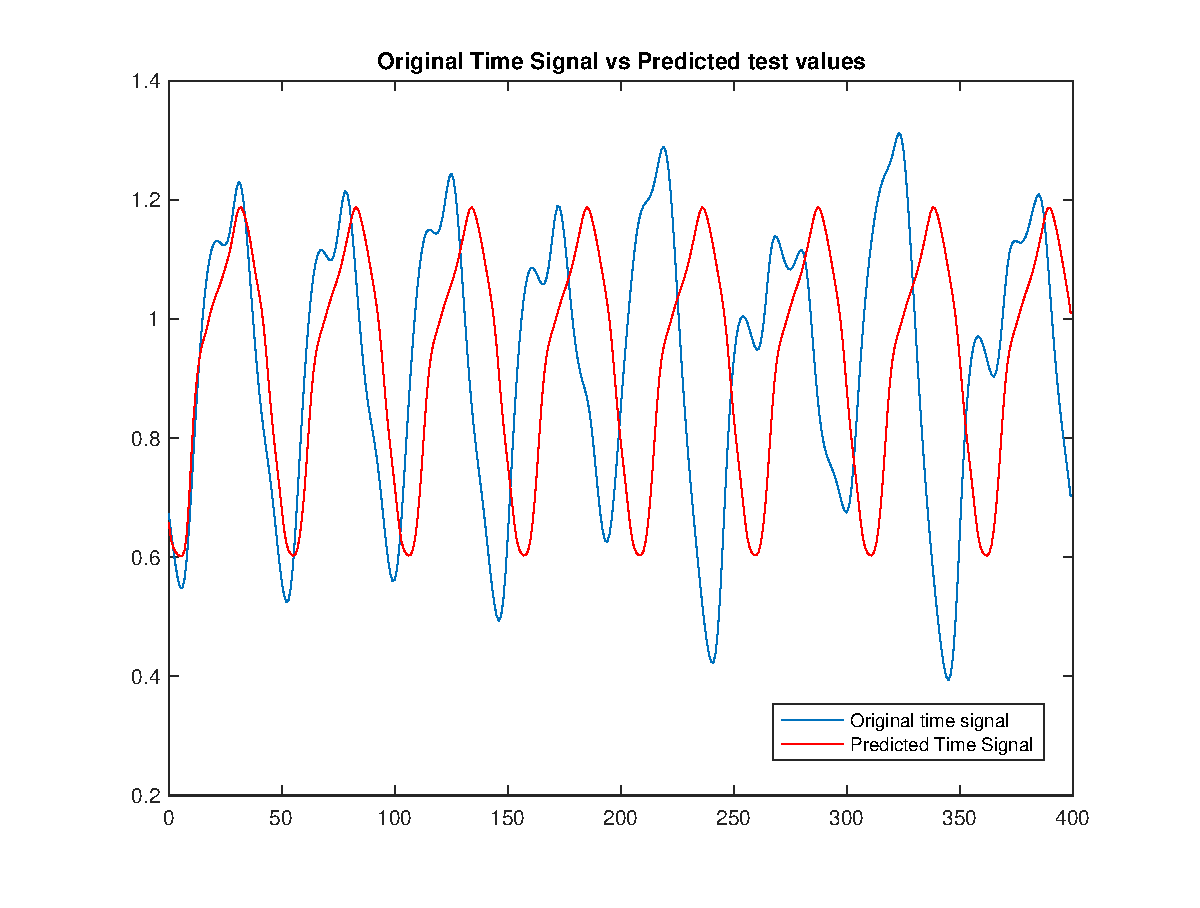
\includegraphics[clip,width=\columnwidth]{figures/PlotTimeSeriesResult}% 
\caption[Graph.]{This is an example of a figure and its caption.}
\label{fig:timeseries}
\end{figure}

\begin{table}[!ht]
\renewcommand{\arraystretch}{1.50}
\caption{This is an example of a table and its caption.}
\label{tablePCA}
\centering
\begin{tabular}{| c | c |}
\hline
\bfseries PCA & \bfseries Residual mean (in absolute values) \\
\hline\hline
Original PCA & 0.1267  \\
\hline
PCA on Centroid 1 & 0.1249\\
\hline
PCA on Centroid 2 & 0.1214  \\
\hline
\end{tabular}
\end{table}

\newpage



%Discussion
\chapter{Discussion}

XXXXXXXXXXX

\section{Discussion}

XXXXXX

Too little representation layer?

\begin{figure}
    \centering
    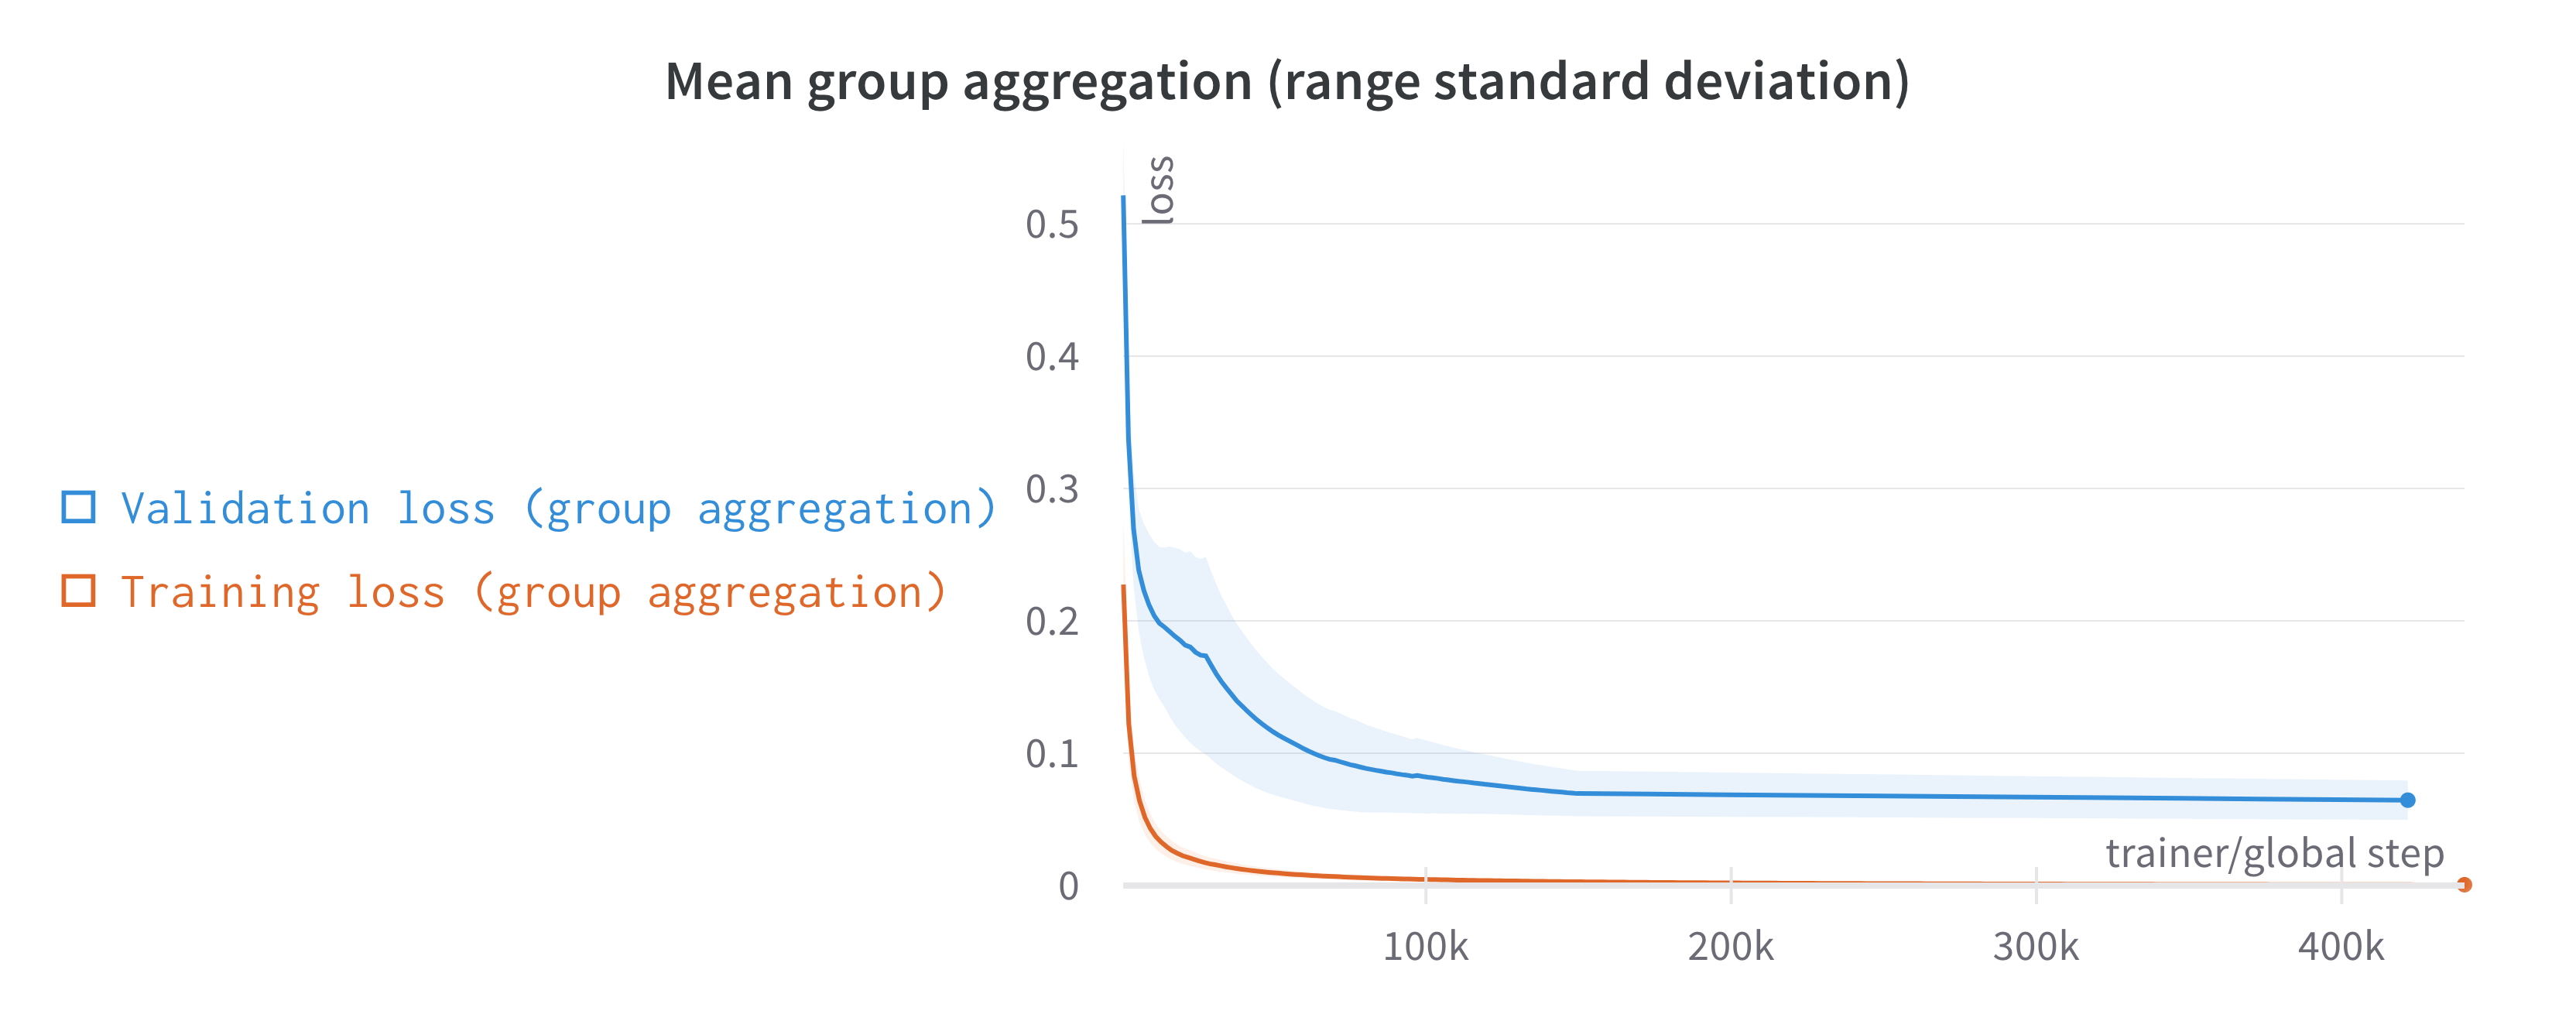
\includegraphics[width=\textwidth]{figures/images/Mean group aggregation.png}
    \caption{Caption}
    \label{fig:enter-label}
\end{figure}

\section{Conclusions}

In this work, we introduced a method to uncover underlying high-level musical
content in the temporal domain by leveraging self-supervised deep neural networks to learn low-dimensional music latent representations with applications to music boundary detection. Building on existing approaches and architectures, we replaced traditional features with deep embeddings trained to represent high-level musical content information.

\newpage



%Future work
\chapter{Future Work}

The question as per \cite{Turian2022HEAR:Representations} or \cite{Li2023MERT:Training} remains if such general-purpose audio representation can mimic human hearing. That is a "thorn in our side" that we will pursue.

\begin{itemize}
  \item Transforms
  \item Stems
  \item Different takes
  \item k-fold cross validation
  \item Hyper-params: kernel size $0.005$ times the sample rate
  \item Larger representation layer
  \item Easy triplet mining \cite{XuanImprovedMining}
  \item Different boundary detection algorithms \cite{sf} was used because it was the default in MSAF \cite{MSAF}
\end{itemize}

Loss function margin. A margin of 0.2 can be a starting point, but it might not be the best value for every task. It's recommended to experiment with different values and choose the one that provides the best performance on your validation set.

Utilize the dB-scale Mel-spectrum magnitude of audio as input data; it is a popular choice for input representation in music-related tasks when applying CNNs, as has been demonstrated in various studies \cite{Kim2020OneStrategies}. While raw audio is the most meaningful audio representation, it's been reported that dB-scale Mel-spectrum frequency-domain summarization, grounded in psycho-acoustics, is computationally efficient and challenging to replicate solely through data-driven methods \cite{Kim2020OneStrategies}; therefore, a trade-off that looks worthy of being explored.

Visual and listening evaluation: 2D or 3D latent space visualization as per \ref{fig:manifold}. Arranging the embedding space in a visual display to evaluate the clustering of this sophisticated musical content to see to what extent they consider sonic attributes. 

\begin{figure}[ht]
    \centering
    \scalebox{1.2}{

\begin{tikzpicture}
\centering
\draw[->] (0, 0) -- ++(0, 2);
\draw[->] (0, 0) -- ++(2.5, 0.6);
\draw[->] (0, 0) -- ++(3, 0) node[midway, below, yshift=-0.5em]
    {Original space ${\cal X}$};

\draw[fill=green!50, draw=none, shift={(0.2, 0.7)},scale=0.5]
  (0, 0) to[out=20, in=140] (1.5, -0.2) to [out=60, in=160]
  (5, 0.5) to[out=130, in=60]
  cycle;

\shade[thin, left color=green!10, right color=green!50, draw=none,
  shift={(0.2, 0.7)},scale=0.5]
  (0, 0) to[out=10, in=140] (3.3, -0.8) to [out=60, in=190] (5, 0.5)
    to[out=130, in=60] cycle;

  \draw[->] (4.8, 0.8) -- ++(0, 2);
  \draw[->] (4.8, 0.8) -- ++(2, 0) node[midway, below, yshift=-0.5em]
      {Latent space ${\cal F}$};

  \draw[thin, fill=green!30, draw=none, shift={(5.4, 1.1)}, rotate=20]
    (0, 0) -- (1, 0) -- (1, 1) -- (0, 1) -- cycle;

  \draw[thick,->,red]
    (1.5, 1.3) to [out=55, in=150] node[midway, above, xshift=6pt, yshift=2pt]
    {$f$} (5.7, 2);

  \draw[thick,->,blue] (1.5, 1.3) ++(4.03, 0.3) to [out=150, in=55]
    node[midway, below, xshift=2pt, yshift=-2pt] {$g$} ++(-3.6, -0.5);

\end{tikzpicture}}
    
    \caption[Dimensionality reduction and latent space representation \cite{tikz}.]{\small{Dimensionality reduction and latent space representation: Mapping between the original high-dimensional space ${\cal X}$ and the lower-dimensional latent space ${\cal F}$ using functions $f$ and $g$.}}
    \label{fig:manifold}
\end{figure}


\newpage
\newpage

\listoffigures
\newpage
\listoftables

% appendices come here
\bibliographystyle{naturemag}
\bibliography{bibliography/references.bib}

\newpage
\appendix
\chapter{Appendix} %Appendix A

Insert python code

\chapter{Appendix} %Appendix B

\chapter{Appendix} %Appendix C

\newpage


\end{document}